\chapter{Article 3 - Evolutionary mechanisms driving the loss of the intromittent phallus in avian lineages}
\label{IPLOSS}

\begin{center}
 \large Alexandre Laverré$^{\text{1}}$, Maëva Luxey$^{\text{1}}$, Patrick Tschopp$^{\text{2}}$, Anamaria Necsulea$^{\text{1}}$\\
 \vspace{0.5cm}
 \normalsize
 $^{\text{1}}$Univ Lyon, Université Claude Bernard Lyon 1, CNRS, Laboratoire de Biométrie et Biologie Evolutive, F-69100, Villeurbanne, France.\\
 $^{\text{2}}$Laboratory of Regulatory Evolution, DUW Zoology, University of Basel, Basel CH-4051, Switzerland\\
\end{center}

{\hypersetup{linkcolor=GREYDARK}\minitoc}

\section{Abstract}
The intromittent phallus (IP), which is thought to provide an important reproductive advantage in terrestrial organisms, was independently reduced or lost in multiple avian lineages. The molecular mechanisms that led to this important morphological change are not yet understood, but are thought to involve gene expression modifications in the pathways that control apoptosis. Here, we investigate the genetic basis of this major phenotypic change through a comparison of gene expression patterns and regulatory element activity during the development of genital tubercles in duck (which has retained an IP) and chicken (which has undergone complete IP loss). We show that broad gene expression patterns are overall conserved between the two species but we also we identify numerous differences in the temporal activity of developmental transcription factors between the two species. We examine the patterns of sequence evolution of putative genital tubercle enhancers across the avian phylogeny and we show that many of these elements independently underwent accelerated evolution in species that lack an IP. Although we cannot pinpoint the molecular causes of the IP reduction/loss, our work brings important insights into the common genomic consequences that followed this convergent phenotypic change in multiple avian lineages.

\section{Introduction}
The vertebrates’ transition from aquatic environments to life on land, more than 300 million years ago, was accompanied by multiple morphological and physiological adaptations. One of these adaptations is internal egg fertilization, which represents an important reproductive advantage for terrestrial organisms. This mode of reproduction is facilitated by the presence of an intromittent phallus (IP), which helps sperm delivery to the ovule. However, although an intromittent male reproductive organ was likely present in the ancestor of all amniotes \citep{brennan_evolution_2016}, the IP was reduced or entirely lost in multiple avian lineages \citep{herrera_developmental_2013}. The evolutionary processes that led to phallus reduction or loss in these species, which nevertheless retained internal fertilization, are still unclear. Given that mating with males lacking an IP requires female cooperation and thus allows females more control over fertilization, one hypothesis posits that this process occurred as a result of sexual selection through female choice of mates \citep{briskie_sexual_1997}. It was also proposed that IP loss was a consequence of natural selection, as it reduced the risk of sexually transmitted diseases in species with a cloaca, which is a common passage for the urogenital and gastrointestinal systems \citep{briskie_sexual_1997}. \\

The developmental processes and molecular mechanisms that are responsible for IP reduction or loss are also not yet fully understood. At early developmental stages, the genital tubercles of birds lacking an IP are morphologically similar to those of birds with an IP, but later on they undergo massive cell death, which leads to a substantial reduction of the male genitalia in these lineages \citep{herrera_developmental_2013}. This earlier activation of apoptosis signals, compared to the mouse model and to bird species that retained an IP, appears to be driven by a temporal gain in the expression of \textit{BMP4}, a developmental transcription factor that can induce cell death in multiple contexts \citep{herrera_developmental_2013}. The genetic basis of this evolutionary change in gene expression is unknown, and so are its implications at the level of the entire transcriptome. It is also not clear whether the same molecular changes occurred in all the lineages in which the IP was lost or reduced.\\

The molecular and evolutionary underpinnings of this morphological transformation are further complicated by the fact that the genes involved in genital development are highly pleiotropic. This is the case for posterior \textit{HOX} genes, which are essential for both limb and genital development in mammals \citep{mortlock_mutation_1997}. Moreover, many of the regulatory elements that control developmental gene expression are shared between limbs and genitalia \citep{lonfat_convergent_2014,infante_shared_2015}. A non-adaptive mechanism for IP reduction/loss can thus be envisaged, as a side-effect of evolutionary changes in other anatomical structures with shared developmental mechanisms. In particular, we note that convergent morphological evolution also affected the limbs in avian species, for example with respect to the loss of the ability to fly \citep{sackton_convergent_2019}. It is not yet clear if these two processes are to some extent inter-connected. \\

Many questions thus remain open regarding the evolutionary processes and the molecular mechanisms that drive the convergent reductions or losses of the intromittent phallus in avian lineages. The increasing accessibility of technologies that assay gene expression and regulation \citep{buenrostro_transposition_2013,wang_rna-seq_2009}, as well as the recent publication of numerous avian genome sequences \citep{feng_dense_2020}, offer an opportunity to address these questions at an unprecedented scale. Here, we use RNA sequencing (RNA-seq) to measure gene expression in embryonic genital tubercles across three comparable developmental stages in chicken and duck. We compare expression profiles between species and we uncover substantial differences in the temporal expression profiles of important developmental transcription factors, including some posterior \textit{HOX} genes. We are thus able to extend and enrich the previously proposed model for gene expression changes that may underlie IP reduction in the chicken \citep{herrera_developmental_2013}. We also assay the activity of putative regulatory elements using ATAC-seq during genital tubercle development in the two species. We analyze the patterns of sequence evolution of enhancer elements predicted with ATAC-seq data. We specifically searched for regulatory elements whose sequences evolve rapidly, independently in multiple avian lineages that underwent IP reduction or loss. We identify numerous such elements and we show that they tend to be located close to genes whose homologues are involved in genital development in the mouse model. We cannot claim that these changes in regulatory programs are causal to the change in phenotype. However, at the very least, these instances of accelerated evolution of regulatory elements illustrate the genome-wide consequences of this major phenotypic change \citep{hiller_forward_2012}, which include widespread relaxation of selective pressures on elements functioning exclusively in genital development. 


\section{Results}

\subsection{Global similarity of gene expression patterns during the development of external genitalia in chicken and duck}

A previous comparative analysis of expression patterns for candidate genes revealed that the developmental transcription factor \textit{BMP4} is activated early and strongly in the chicken genital tubercle, compared to duck and to the mouse model \citep{herrera_developmental_2013}. To extend this comparative analysis at the genome-wide level, we generated RNA-seq data for the developing genital tubercles of chicken and duck. We selected three time points during embryonic development, defined with the Hamburger-Hamilton (HH) staging system \citep{hamburger_series_1951} as follows: stage HH29, at which the external genitalia development has already started but there are no morphological differences between the two species; stage HH33, at which the genital tubercle begins to degenerate in chicken embryos but continues to grow in duck; and stage HH36, at which genital tubercle development is well advanced in the duck (Figure \ref{fig:IPLOSS-fig-sampling-scheme}).\\ 

\begin{figure}[h]
 \centering
 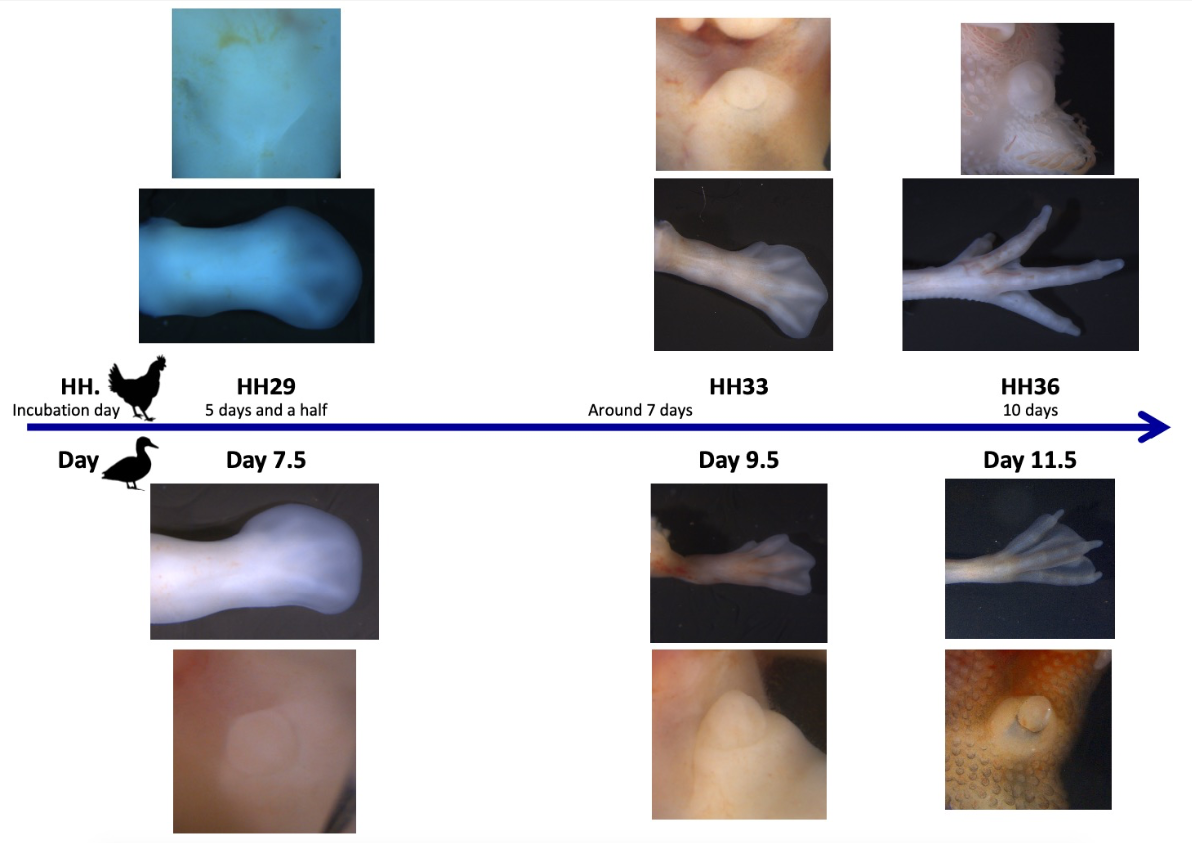
\includegraphics[width=1\textwidth, page=1] {figures/IPLOSS/SamplingScheme.png}
 \caption[Morphology of the developing genitalia and limbs in chicken and duck.]{
 \textbf{Morphology of the developing genitalia and limbs in chicken and duck, at different developmental stages.} The images show photos of representative embryos for chicken (top) and duck (bottom), at three developmental stages: HH stages 29, 33 and 36. Limb morphology was used as a marker to help with the precise identification of corresponding developmental stages in the two species. \\
 }
 \label{fig:IPLOSS-fig-sampling-scheme}
\end{figure} 

Overall, gene expression patterns in the developing genital tubercles are well conserved between chicken and duck, despite the known morphological differences between the two species (Figure~\ref{fig:IPLOSS-fig1}). We clustered samples based on a measure of similarity of their global expression patterns (Spearman's correlation coefficient, computed on TPM expression levels for 12878 genes with 1-to-1 orthologues between chicken and duck). We found that samples were grouped first by species and second by developmental stage, with the two earliest stages (HH29 and HH33) grouped together apart from the later stage (HH36) in each species. Thus, differences between species are the main factor of gene expression variability in our dataset. However, we observed very high levels of similarity even for comparisons across species (Spearman's correlation coefficient above 0.8 in all pairwise comparisons, with a maximum of 0.98 observed across biological replicates). Interestingly, the difference between the later developmental stage and the two earlier ones is more pronounced in chicken than in duck (Figure~\ref{fig:IPLOSS-fig1}A). This may reflect the fact that morphological differences between early and late genital development are more important in chicken (where tubercle growth has stopped by stage HH36) than in duck (where growth continues for a longer time period).\\

\begin{figure}[hbt!]
 \centering
 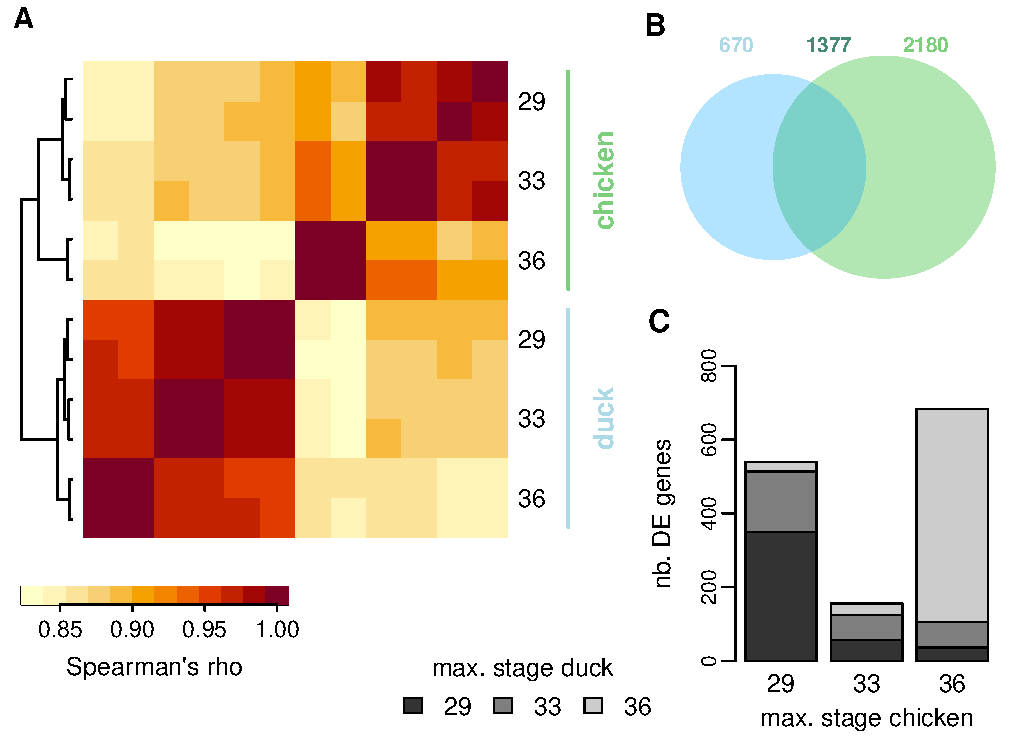
\includegraphics[width=1\textwidth, page=1] {figures/IPLOSS/IPLOSS_Figure1.pdf}
 \caption[Comparison of gene expression patterns during genital tubercle development in chicken and duck.]{
 \textbf{Comparison of gene expression patterns during genital tubercle development in chicken and duck.}
 \textbf{A.} Hierarchical clustering based on pairwise Spearman's correlation coefficients, computed on the TPM expression levels of 12878 genes with 1-to-1 orthologues between chicken and duck. Developmental stages and species labels are indicated on the right side of the plot.
 \textbf{B.} Venn diagram representing the numbers of significantly (FDR $<$ 0.01, fold expression change $\geq$ 1.5) differentially expressed (DE) genes in chicken (green) and duck (light blue).
 \textbf{C.} Comparison between the developmental stage (HH29, HH33 or HH36) in which maximum expression is reached in chicken and in duck, for the 1377 genes that are significantly DE in both species. Genes are divided into three classes depending on the stage with maximum expression in chicken (vertical bars). Within each class, the height of the colored rectangles represents the numbers of genes that reach their maximum expression level in the three developmental stages in the duck. 
 \\
 }
 \label{fig:IPLOSS-fig1}
\end{figure} 

We next evaluated quantitative expression differences among developmental time points, independently for each species (Methods). We observed that large proportions of genes are differentially expressed (DE) with stringent significance criteria (maximum FDR 1\%, minimum fold change 1.5) among stages: 670 genes (5\% of all genes with 1-to-1 orthologues) are DE only in duck, 2180 (17\%) are DE only in chicken and 1377 (11\%) are DE in both species (Figure~\ref{fig:IPLOSS-fig1}B). The proportion of shared DE genes is significantly higher than expected by chance, under the null hypothesis that differential expression is independent between species ($\chi$-squared test, p-value $<1e^{-10}$). Moreover, the 1377 genes that are DE in both species generally reach their maximum expression levels at similar developmental stages in both species (Figure~\ref{fig:IPLOSS-fig1}C).

\subsection{Distinct temporal expression profiles in the developing genitalia of chicken and duck}

Although global gene expression profiles are very similar between chicken and duck, our first analyses already indicate that some genes may have distinct behaviors in the two species. Notably, in some cases the maximum expression level is observed at different time points in the two species (Figure~\ref{fig:IPLOSS-fig1}C). To better identify the genes with distinct patterns of temporal variation in chicken and duck, we first defined relative expression profiles by dividing TPM values (averaged across biological replicates for each developmental stages) by their maximum, for each gene and separately for each species. We then grouped the two profiles obtained for each species, thus obtaining a series of 6 numeric values comprised between 0 and 1 for each pair of 1-to-1 orthologous genes. We clustered these profiles with a k-means approach. The resulting clusters group together genes whose relative expression profiles are similar to one another. There is no requirement of similarity between the two species (Methods). We set the number of different clusters at 9, reasoning that this should allow us to capture most of the variability that exists with only 6 species/time point combinations. 

Among the 9 requested clusters of genes, we observed that 6 could be classified as having similar behaviors between chicken and duck (Figure~\ref{fig:IPLOSS-fig2}). These clusters seem to represent all possible temporal dynamics: rapid increases or decreases during developmental time; more moderate increases or decreases, in which the late developmental stage stands out from the two earlier ones; or a dynamics reaching a peak in the middle developmental stage (Figure~\ref{fig:IPLOSS-fig2}). These clusters already allow us to highlight a surprising pattern: the \textit{BMP4} gene, for which a very different pattern of temporal activation was previously observed between chicken and duck \citep{herrera_developmental_2013}, falls into a cluster showing a gradual increase of expression with time in both species (Figure~\ref{fig:IPLOSS-fig2}). We note that absolute expression levels are difficult to compare between distant species \citep{brawand_evolution_2011}, and we prefer to avoid over-interpreting apparent differences in TPM values (at least when they are as subtle as for \textit{BMP4}). Nevertheless, depending on which time points can be taken as a common reference for the two species, the \textit{BMP4} expression pattern can be interpreted as an earlier activation in chicken than in duck (at stage HH33 rather than at stage 36), consistent with previous observations \citep{herrera_developmental_2013}. However, the differences between chicken and duck are much more subtle than the ones reported previously \citep{herrera_developmental_2013}. \\


\begin{figure}[hbt!]
 \centering
 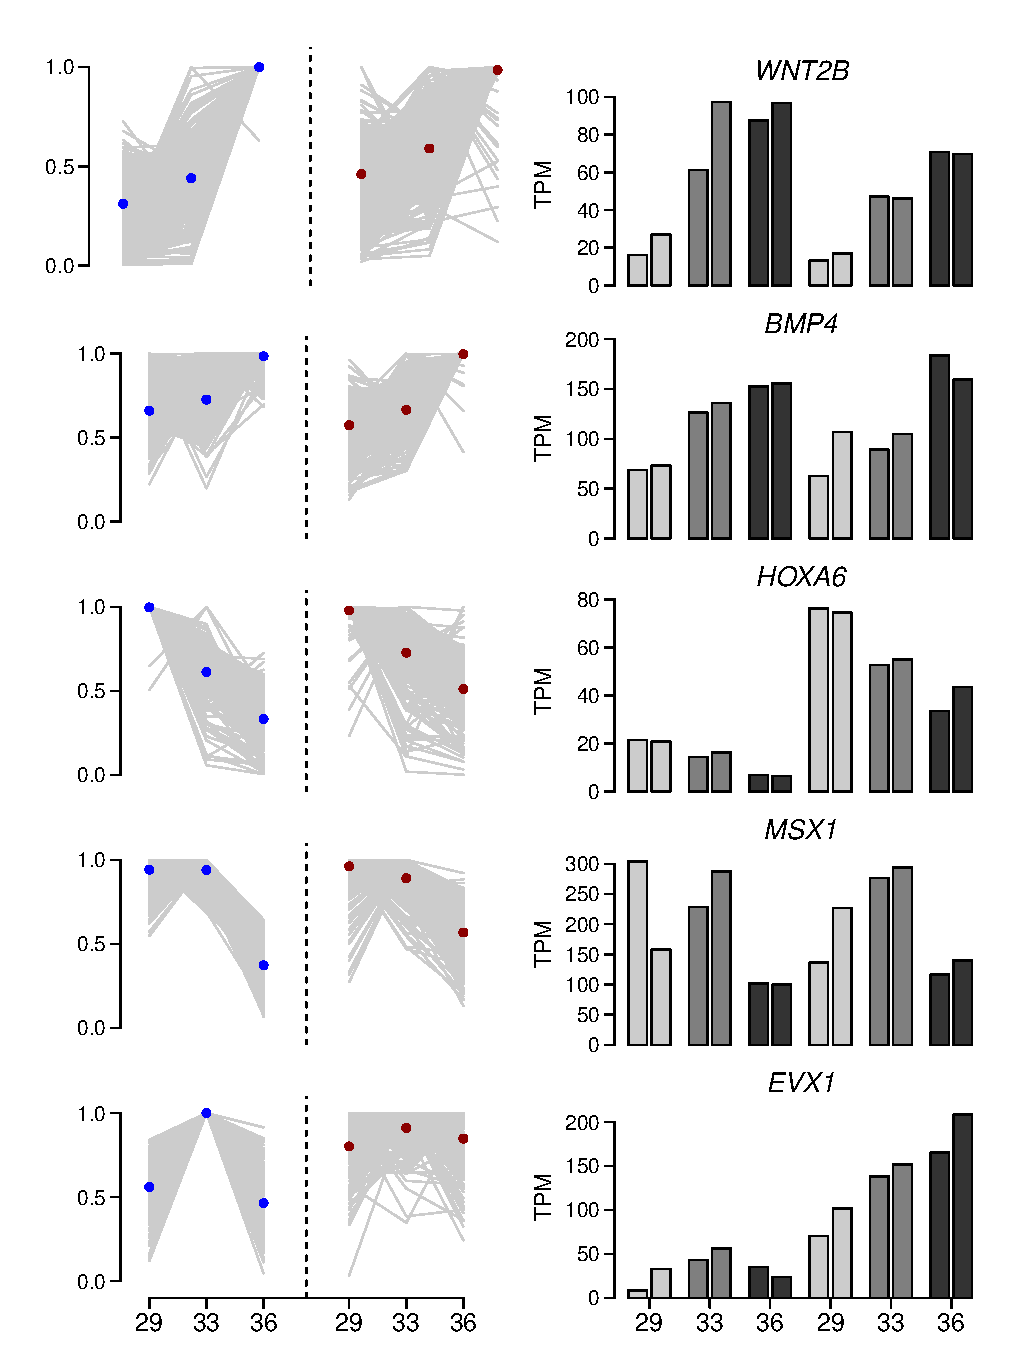
\includegraphics[width=0.9\textwidth, page=1] {figures/IPLOSS/IPLOSS_Figure2.pdf}
 \caption[K-means clustering of relative expression profiles (clusters with similar behavior between chicken and duck).]{
 \textbf{K-means clustering of relative gene expression profiles during the development of chicken and duck genital tubercle.} Each horizontal panel represents one cluster of genes that are similar to one another in terms of relative expression profiles. Expression levels were transformed into relative profiles by dividing by the maximum, separately for each species. Biological replicates were combined into a single average value for the clustering analysis. Blue dots: chicken; red dots: duck. Barplots representing TPM values for all samples are shown on the right hand side of the plot, for one representative gene within each cluster. First 6 vertical bars represent the chicken samples, last 6 bars represent the duck samples.\\
 }
 \label{fig:IPLOSS-fig2}
\end{figure} 

We also observe 3 gene clusters in which the patterns of temporal variation are different between chicken and duck. These clusters include several genes that are known to be implicated in the development of external genitalia in the mouse model. In particular, \textit{HOXD13} shows strikingly different patterns between the two species: in the chicken, \textit{HOXD13} expression decreases with developmental time, while in the duck it rapidly increases (Figure~\ref{fig:IPLOSS-fig3}). Here again, this expression pattern is in disagreement with the one reported in previous work \citep{herrera_developmental_2013}, where \textit{HOXD13} was not seen as expressed in the late developmental stages. 

% Nevertheless, we observe significant differences in temporal expression patterns for key genes involved in the development of external genitalia. For example, posterior HoxD genes (in particular Hoxd13) are highly expressed in duck genitalia and have higher levels of expression in the later developmental stages. In contrast, in the chicken they are more weakly expressed and do not increase with time (Figure \ref{fig:IPLOSS-fig5}). These results are in agreement with a decrease in cell proliferation levels in the chicken phallus precursors.

\begin{figure}[hbt!]
 \centering
 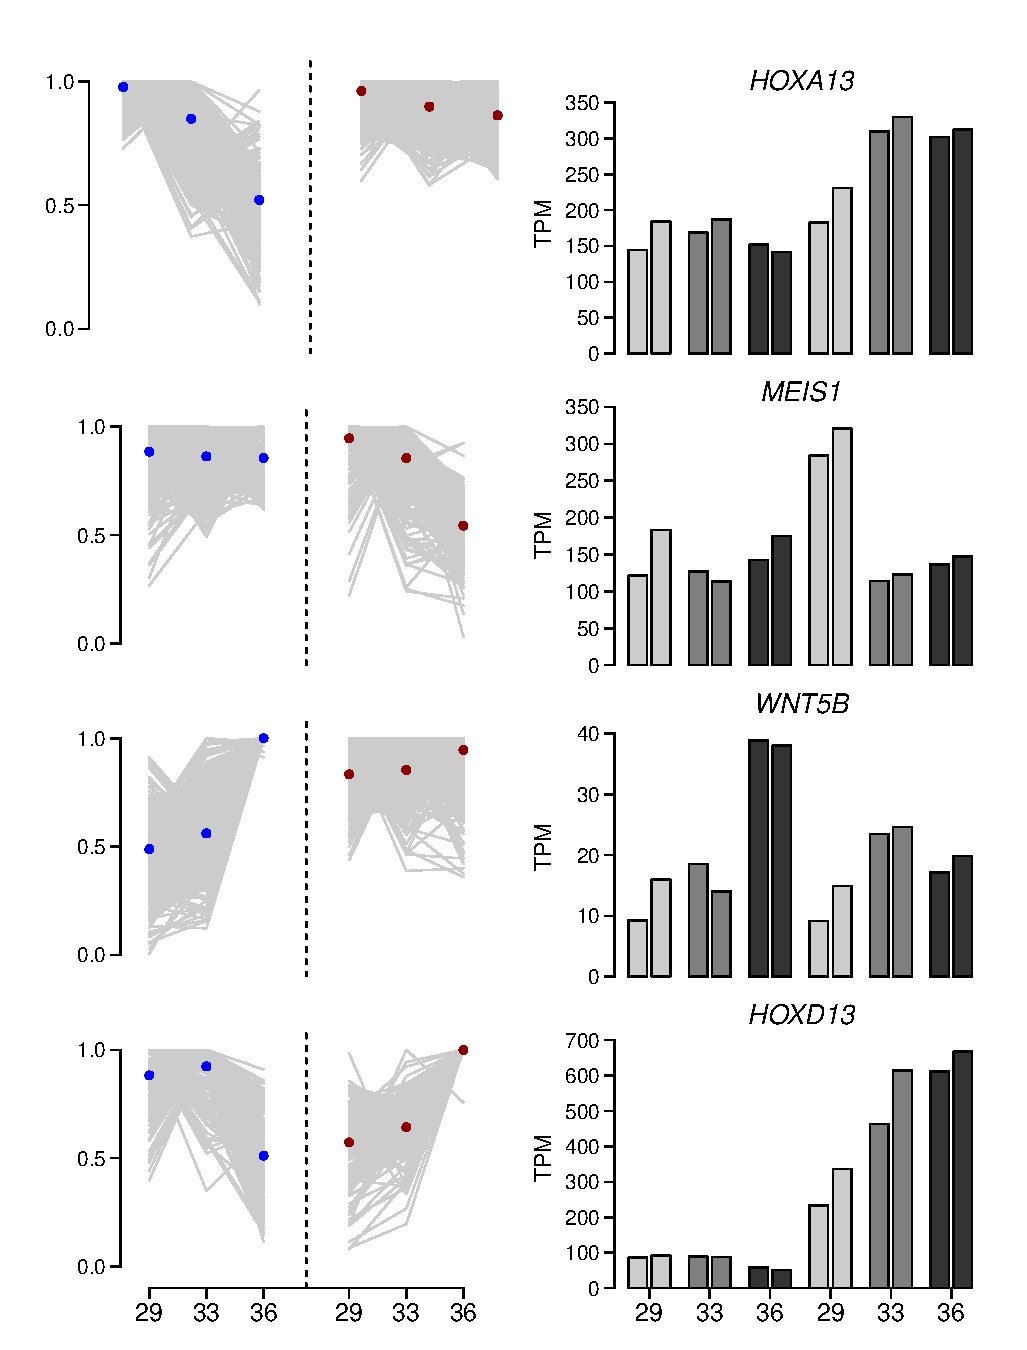
\includegraphics[width=0.9\textwidth, page=1] {figures/IPLOSS/IPLOSS_Figure3.pdf}
 \caption[K-means clustering of relative expression profiles (clusters with similar behavior between chicken and duck)]{
 \textbf{K-means clustering of relative gene expression profiles during the development of chicken and duck genital tubercle.}
 Each horizontal panel represents one cluster of genes that are similar to one another in terms of relative expression profiles. Expression levels were transformed into relative profiles by dividing by the maximum, separately for each species. Biological replicates were combined into a single average value for the clustering analysis. Blue dots: chicken; red dots: duck. Barplots representing TPM values for all samples are shown on the right hand side of the plot, for one representative gene within each cluster. First 6 bars represent the chicken samples, last 6 bars represent the duck samples.
 \\
 }
 \label{fig:IPLOSS-fig3}
\end{figure} 

\subsection{Detection of putative enhancers active during chicken and duck genitalia development}

To predict the regulatory elements that control gene expression during chicken and duck external genitalia development, we generated ATAC-seq data for the developing GT, for embryonic stages HH29 and HH33 in chicken and duck. To identify GT-specific regulatory regions, we complemented this dataset with previously published ATAC-seq data for the two species. These included data for the developing limb, muscle, keel and sternum in chicken \citep{sackton_convergent_2019}, and for adipose and sebum cells in duck \citep{zhu_three_2021}. The numbers of open chromatin regions detected with ATAC-seq data (ATAC-peaks) is heterogeneous between samples (Figure \ref{fig:IPLOSS-fig4}.A). In particular, chicken GT samples show low numbers of peaks (35,725 and 38,394 for stages HH29 and HH33) compared to other samples. The number of non-GT ATAC-peaks in duck are particularly high, likely due to the high sequencing depth available for these samples. To correct for the bias in detection sensitivity that is due to differences in sequencing depth, we resampled the same numbers of ATAC-peaks within each species (Methods). 
To determine putative enhancer elements starting from the ATAC-peaks, we first classified the peaks with respect to genomic annotations. We found that the proportions of exonic, intronic and intergenic regions are not significantly different between samples (Figure \ref{fig:IPLOSS-fig4}.A). We selected intergenic and intronic peaks for further analyses. \\

%% - transcription factors binding site enrichment GT vs other (Methods)

%The number of ATAC-peaks detected in samples are correlated to the sequencing depth (Supplementary Figure, correl test, pval). 

\subsection{Detection and analysis of homologous ATAC-peaks in chicken and duck}

We used a whole-genome alignment to identify homologous ATAC-peaks between chicken and duck (Methods). For each ATAC-peak detected in a given sample, we are thus able to predict whether a homologous sequence exists in the other species and to assess its similarity with the reference sequence. We found that the proportion of ATAC-peaks with predicted homologous regions did not differ between samples, but that the average identity score was significantly lower for chicken GT ATAC-peaks at stage HH29 (Figure \ref{fig:IPLOSS-fig4}.B). \\

For each ATAC-peak for which we could predict a homologous region, we asked whether its predicted homologue overlapped with an ATAC-peak of the other species (Methods). To obtain a first overview of the broad patterns of sequence and open chromatin state conservation, we constructed a matrix consisting of N rows and k columns, where N is the total number of ATAC-peaks detected in the chicken, and the k is the total number of ATAC-seq samples available across both species. This matrix contains for each element and for each sample a value of 0 or 1, depending on whether the element (or its predicted homologue) overlapped with an ATAC-peak in the corresponding sample. A factorial correspondence analysis performed on this table separates the samples by species of origin (Figure \ref{fig:IPLOSS-fig4}.C). The chicken GT ATAC-peaks are closest to those obtained in cells of forelimb and hindlimb development. This result is consistent with the presence of common regulatory programs during the development of these organs in mouse \citep{lonfat_convergent_2014}. Duck GT ATAC-peaks are more similar to chicken GT ATAC-peaks than to other chicken ATAC-peaks. We also found that more than 20\% of the duck GT ATAC-peaks that have homologues in the chicken are also active in the chicken GT (Figure \ref{fig:IPLOSS-fig4}.D). Less than 15\% of the duck non-GT ATAC-peaks have homologues with activity in any of the chicken samples.

\begin{figure}[hbt!]
 \centering
 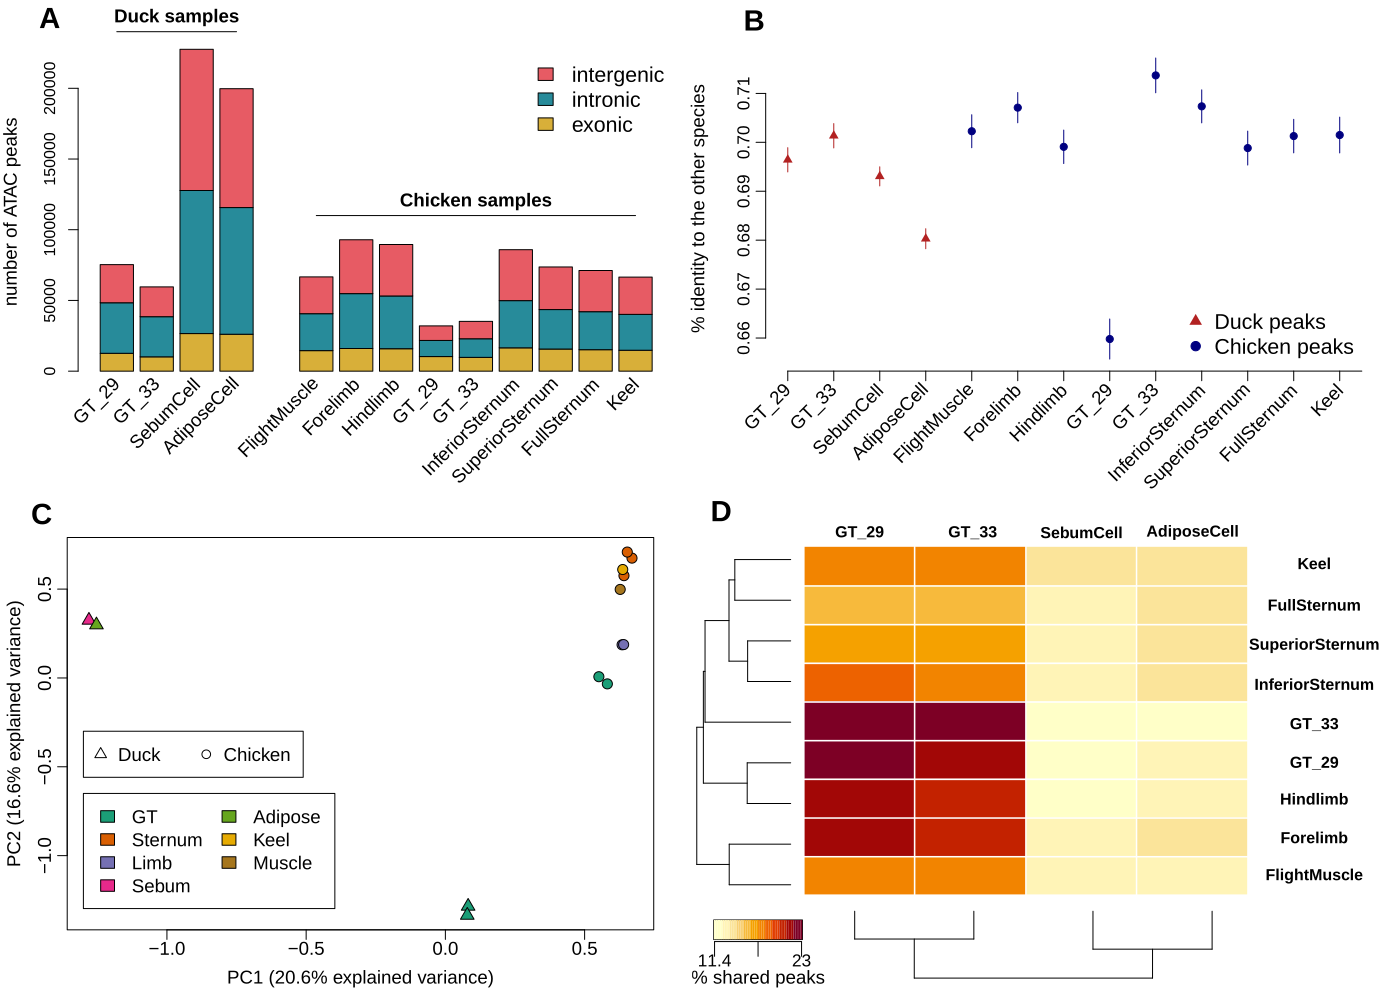
\includegraphics[width=1\textwidth, page=1] {figures/IPLOSS/new_figIPLOSS2.png}
 \caption[Comparison of ATAC-seq data in duck and chicken samples.]{
 \textbf{Comparison of ATAC-seq data in duck and chicken samples.}
 \textbf{A.} Distribution of the number of ATAC-peaks detected in duck and chicken samples. Peaks are classified according to their overlap with exons (exonic, yellow), introns (intronic, blue) or intergenic regions (intergenic, red). 
 \textbf{B.} Distribution of the median percentage identity between sub-sampled duck ATAC peaks sequences (N=63,250) aligned in the chicken genome (red triangle), and between sub-sampled chicken ATAC peaks sequences (N=35,725) aligned in the duck genome (blue circle). Error bars represent the 95\% confidence interval of median. 
 \textbf{C.} Factorial correspondence analysis of chicken and duck samples based on homologous subsampled peak activity. Homologous sequences of peaks from a reference species are active in the target species if they overlap at least one base of an ATAC peak in this species (Methods). \textbf{D.} Proportion of subsampled duck ATAC peaks whose homologous sequence overlaps with an ATAC peak in the chicken samples. Dendrograms are produced from the ATAC peak activity binary matrix of each species. \\
 }
 \label{fig:IPLOSS-fig4}
\end{figure} 

\subsection{Regulatory sequence evolution in bird lineages}

Regulatory elements that control gene expression exclusively in the IP are expected to display accelerated evolution in the lineages where this organ was lost, due to relaxation of purifying selection. Evolutionary sequence analyses can thus help identify elements that function in this organ. We analysed the rates of sequence evolution of all non-exonic ATAC peaks detected in duck (N=171,789) and chicken (N=264,331), by aligning them with their putative homologues in the genomes of 53 bird species (Figure \ref{fig:IPLOSS-fig5}.A; Methods). We repeated this analysis   starting from a set of conserved non-coding sequences defined from an alignment between muscovy duck (\textit{Cairina moschata}) and other birds with an IP (Methods). \\

%Of these species, 21 possess an IP and the phylogenetic distribution of this phenotype would represent 5 independent convergent losses \citep{brennan_independent_2008}. \\

We computed the rates of sequence evolution in each lineage and for each input element with phyML and we estimated relative evolutionary rates within each lineage (Methods). A high relative evolution rate in a lineage indicates an accelerated divergence of the sequence relatively to all other analysed sequences. For each alignment, we estimated the correlation between the relative evolutionary rates and the distribution of the IP presence/absence phenotype along the phylogeny (Figure \ref{fig:IPLOSS-fig5}.B; Methods). A negative correlation coefficient indicates that the sequence underwent a convergent acceleration of its evolutionary rate in species with a reduction or loss of the IP. Conversely, a negative correlation coefficient indicates that higher relative rates of evolution are associated with species that have an IP.   The duck ATAC-peak that has the strongest association with the IP phenotype has a median relative evolutionary rate of -1.12 in species with IP and 0.35 in species without (Rho=-0.49 ; FDR=5.2e-3). The proportion of sequences whose evolutionary rates are significantly associated with the IP phenotype is low for all tested datasets (Figure \ref{fig:IPLOSS-fig5}.C; median across duck samples = 0.53\%). 
Among ATAC-peaks that are significantly associated with the IP phenotype, there is an enrichment for peaks that evolve faster in species without an IP (mean across samples 82\% , $\chi$-squared test, p-value $<1e^{-10}$). The proportion of ATAC-peaks that are correlated with the IP phenotype varies depending on the tissue in which the peaks are active. For duck ATAC-peaks, a larger fraction of sequences are accelerated in non-IP species in GT (0.48\% and 0.51\% in stages HH29 and HH33 respectively) than in the other tissues (0.37\% and 0.39\% in sebum and adipose cells) ($\chi$-squared test, p-value=2e-07). We detected 535 sequences whose rates of evolution are significantly correlated with the IP phenotype, among duck GT ATAC-peaks. For 25\% of these peaks, we found homologous chicken ATAC-peaks and conserved non-coding sequences that also had accelerated rates of evolution (Figure \ref{fig:IPLOSS-fig5}.E).\\

To further test the significance of the results, given the sparse distribution of the "with IP" phenotype along the phylogeny, we performed random permutations of the phenotype and repeated the analyses (Figure \ref{fig:IPLOSS-fig5}.D). The median of the observed absolute correlation coefficients (median=0.09) is significantly higher than in the random permutations (median permutations=0.06, FDR $<1e^{-5}$). Furthermore, the average number of ATAC peaks correlated with the presence of an IP in the random permutations is significantly lower (4.7) than the one observed for the distribution of true phenotypes (1300, FDR $<1e^{-5}$).


\begin{figure}[hbt!]
 \centering
 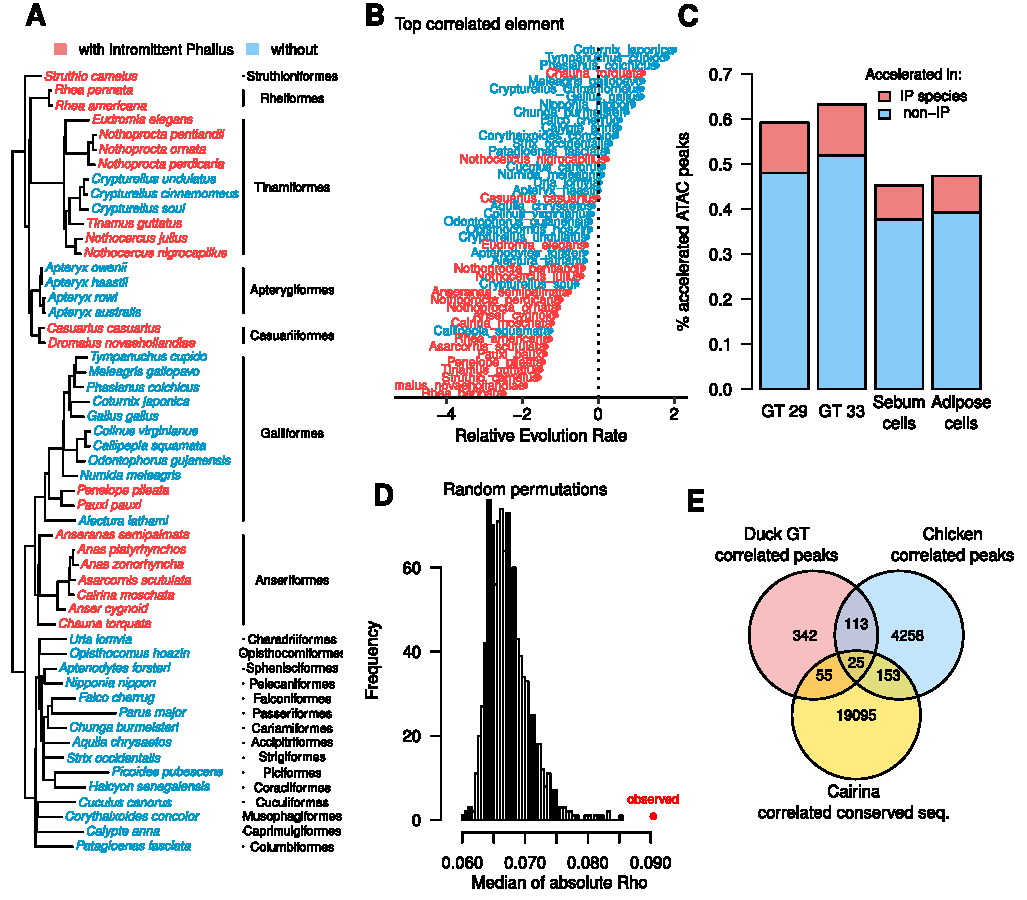
\includegraphics[width=0.9\textwidth, page=1] {figures/IPLOSS/Fig_evol_peaks.pdf}
 \caption[Enrichment for convergently accelerated sequences in birds that lost the intromittent phallus.]{
 \textbf{Enrichment for convergently accelerated sequences in birds that lost the intromittent phallus.}
 \textbf{A.} Species tree. Species names are coloured according to the presence (red) or absence (blue) of an intromittent phallus (IP). The Order to which the species belong is indicated. Obtained from the species tree of \citep{feng_dense_2020}. 
 \textbf{B.} Example of the relative evolution rate distribution among species estimated by RERconverge, for the duck ATAC-peak that is the most correlated with the presence of the phallus \citep{kowalczyk_rerconverge_2019}. Species with IP are associated with lower relative evolution rates than species without IP for this sequence (Rho=-0.49 ; FDR=5.2e-3). 
 \textbf{C.} Proportion of sequences whose rate of evolution is correlated with the presence of IP among ATAC data from duck samples. Accelerated sequences in species with an IP are shown in red and accelerated sequences in non-IP species in blue.
 \textbf{D.} Distribution of the median correlation coefficients between the relative evolution rate of duck ATAC-peaks and the presence of the IP based on 1000 random permutations of the phenotype in the phylogeny. The observed value for the actual phenotype distribution (A.) is shown in red. 
 \textbf{E.} Overlap of homologous sequences correlated with the presence of IP depending on whether they are from duck ATAC data (red), chicken ATAC data (blue) or muscovy duck non-coding sequences conserved in species with an IP (yellow). \\
 }
 \label{fig:IPLOSS-fig5}
\end{figure} 

\subsection{Accelerated sequences are found near genes involved in GT development}
To asses the biological significance of the putative regulatory elements that show accelerated rates of evolution in species that have lost an IP, we analyzed their putative target genes. 
We predicted their target genes using a genomic proximity approach similar to that implemented in GREAT \citep{mclean_great_2010} (Methods). Duck ATAC-peaks with accelerated evolutionary rate in species without an IP were attributed to genes functionally enriched in developmental processes (consisting of for exemple \textit{AR} and \textit{HOXC10}), response to growth factor (e.g: \textit{EGFR}, \textit{BMP2}), but also to male genitals and tube development (e.g: \textit{SHH}, \textit{PDGFRA}, \textit{BMP6}) (Figure \ref{fig:IPLOSS-fig6}.A). The 25 sequences commonly identified as accelerated in non-IP species from the three datasets (chicken, duck and muscovy duck) are notably associated with two regulatory genes of the Hippo pathway. This signaling pathway modulates cell proliferation, cell death, and cell differentiation \citep{yu_hippo_2013}. \\

We also asked whether some genes are associated more frequently than expected with accelerated sequences (Figure \ref{fig:IPLOSS-fig6}.A). Several genes show higher numbers of accelerated elements in their vicinity than expected by chance (Methods). Thse include the Fibroblast growth factor 5 (\textit{FGF5}) and Epidermal growth factor receptor (\textit{EGFR}). These genes are involved in genital development \citep{ogino_external_2001, harada_tissue-specific_2015}. 
%Finally, we assessed the presence of transcription factor binding sites within accelerated duck ATAC peaks in non-IP species. These sequences show an enrichment of motifs recognised by several developmental genes like HoxD13, HoxC11 relative to all duck peaks.

\begin{figure}[hbt!]
 \centering
 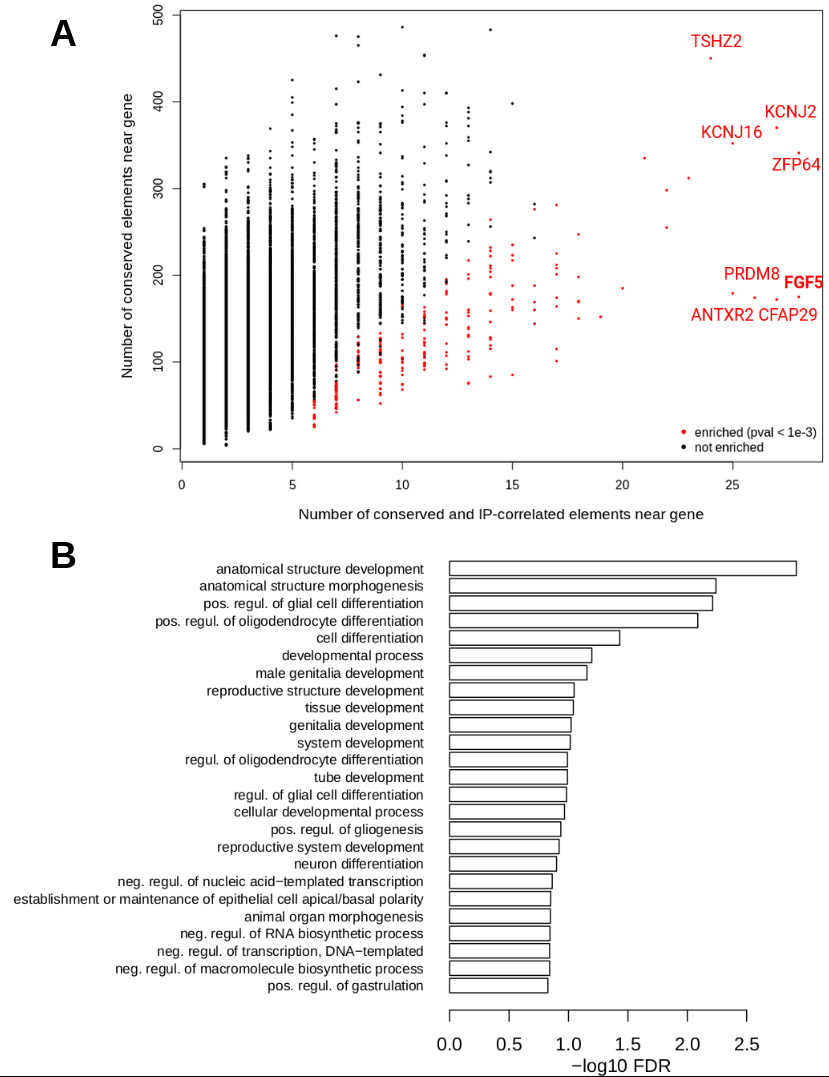
\includegraphics[width=0.9\textwidth, page=1] {figures/IPLOSS/test.png}
 \caption[Detection of genes associated with convergently accelerated sequences in species without an IP.]{
 \textbf{Detection of genes associated with convergently accelerated sequences in species without an IP.}
 \textbf{A.} Enrichment of convergently accelerated elemnts in the vicinity of genes. Each point is a gene represented by the total number of elements and the number of accelerated elements in its neighborhood. Colored points are genes with an excess of convergently accelerated elment based on a permutation test (5\% FDR). Only genes associated with at least one accelerated sequence are plotted. 
 \textbf{B.} Gene Ontology enrichment of genes associated with convergently accelerated duck ATAC-peaks. Only the 25 most enriched terms are shown ordered by FDR value.
 \\
 }
 \label{fig:IPLOSS-fig6}
\end{figure} 

\section{Discussion}
In this work, we aimed to investigate the genetic determinants of the loss of the intromittent phallus, which occurred convergently in multiple avian lineages. We first observed that the vast majority of genes show conserved expression patterns in the genital tubercle between chicken and duck. This observation is in agreement with many studies showing that gene expression evolves slowly, especially during in embryonic development \citep{brawand_evolution_2011, cardoso-moreira_gene_2019}(Tschopp et al. 2014).  The genes involved in the development of the genitalia are known to be pleiotropic. Indeed, studies from mouse and humans showed that numerous master regulatory of embryonic development are involved in both phallus and limb formation \citep{lonfat_convergent_2014,infante_shared_2015}. \\
%However, in view of the major phenotypic change, where the genital tubercle continues to develop in the duck and is reduced in the chicken, we would have expected more difference. 

Nevertheless, some genes do show different or even opposite temporal expression patterns in the two species. These include some crucial developmental genes, such as \textit{HOXD13}, which is known to play an important role in genital development in mouse and humans \citep{dolle_hox-4_1991, klonisch_molecular_2004}. These genes could be good candidates to explain this phenotypic change but further work is needed to confirm their role. Interestingly, we were unable to confirm the candidate genes that were previously proposed to explain this phenotype. For example, \textit{BMP4}, which may play a role in triggering apoptosis in chicken genital tubercle development \citep{herrera_developmental_2013}, in our data shows only subtle differences of expression between chicken and duck, contrary to what was reported. However, we note that with our bulk RNA-seq approach we cannot assess spatial patterns of gene expression, but only have access to the average expression level in the dissected tissue. This could explain part of the difference with previous work. We thus need to confirm our results for interesting candidate genes with \textit{in situ} hybridization approaches.\\

%This can be explained by the fact that we only considered qualitative differences based on relative expression patterns.
%Variations in expression levels between species are not detectable in this way if they follow the same temporal trajectory during development. %It would therefore be interesting to analyse whether such quantitative differences are relevant to the development of the reproductive tract or whether they are simply relative to the species in a broader context. Comparing the expression patterns of genes involved in the development of similar morphological structures such as limbs could provide some answers.\\

We then attempted to detect the \gls{cis}-regulatory sequences that are involved in genital development in birds. We generated  ATAC-seq data to evaluate the presence of open chromatin regions during the development of the genital tubercle in chicken and duck. Phenotypic losses should be followed by a relaxation of selection pressures on those sequences that are exclusively involved in the development and maintenance of these traits. We have detected sequences whose rate of evolution is correlated with the presence/absence of the IP in bird lineages. The open chromatin regions specific to the genital tubercle in ducks are particularly enriched in sequences whose rate of evolution are correlated with the phenotype. These sequences are predominantly accelerated in species who lack an IP, but interestingly we also detect regions with accelerated evolutionary rates in IP species. Further analysis is nevertheless needed to identify the evolutionary reasons that explain these accelerations.\\

The convergently accelerated regulatory sequences in species without an IP are in the vicinity of genes enriched for male genitalia developmental functions, such as \textit{SHH}, \textit{PDGFRA} and \textit{BMP6}, but also developmental genes important in cell growth and differentiation (\textit{HOXC10}, \textit{BMP2}, \textit{AR}). Some of these genes such as \textit{EGFR} and \textit{FGF5} are also enriched in accelerated sequence in their vicinity. These genes and putative regulatory sequences are therefore of particular interest with regard to phallus development in birds. Further analyses are needed to test the regulatory potential of these sequences and their activity pattern in the genital tubercle. Furthermore, joint analyses between the gene expression differences and the detected convergent accelerated sequences are needed to better understand their relationship and to propose mechanisms involved in phallus reduction. Nevertheless, our comparative genome-wide analyses have allowed us to investigate more broadly the molecular mechanisms that may be responsible for this major morphological change in birds.

\section{Methods}

\subsection*{Biological sampling}
We dissected the developing genital tubercles of chicken and duck at Hamilton-Hamburger stages 29, 33 and 36. Two biological replicates were generated for each species and for each developmental stage. Precise embryonic staging was achieved by analyzing the morphology of the limb. Embryos were sexed and only males were used for experiments. The tip of genital tubercle was dissected and used for RNA extraction. A single embryo was used for each extraction. 

\subsection*{Transcriptome sequencing}
We generated transcriptome sequencing (RNA-seq) data for the three developmental stages listed above using the Illumina TruSeq Stranded mRNA protocol. Libraries were sequenced as single end, 100 bp reads, on an Illumina NextSeq 500 machine. Between 30 and 50 million reads were generated for each sample.

%\subsection*{De novo transcriptome annotations}
%We performed de novo transcriptome annotations to improve the protein-coding and non-coding RNA gene repertoire of chicken and duck. We used GeMoMa, a homology-based gene prediction that combines annotations of multiple reference genomes and RNA-seq experiments to infer gene annotations of a target genome. We annotated the genomes of chicken (\textit{Gallus gallus} version Galgal6) and duck (\textit{Anas platyrhynchos platyrhynchos} version CAU\_duck1.0) by using gene annotations of X reference species (including the known annotations of chicken and duck) obtained from Ensembl (version 103) (ref). These annotations resulted in X one-to-one orthologous protein-coding genes used in further analyses.

\subsection*{Gene expression quantification and differential expression}
Gene expression quantification was performed using \texttt{kallisto} version 0.46 \citep{bray_near-optimal_2016} based on Ensembl annotations, version 103 \citep{cunningham_ensembl_2019}. We assessed differential expression among developmental stages in each species with DESeq2 \citep{love_moderated_2014}. Differential expression analyses were performed only on 1-to-1 orthologous genes, as annotated in Ensembl Compara \citep{cunningham_ensembl_2019}. We selected genes that were significantly diferentially expressed in at least one species (false discovery rate 0.01, minimum fold expression change 1.5). We computed relative expression profiles for these genes by first averaging expression levels across replicates, and then dividing each value by the maximum observed across stages, for each gene and separately for each species. We combined the species-specific relative expression profiles obtained for each pair of 1-to-1 orthologous genes, thus obtaining a set of 6 numeric values, corresponding to the 6 species/developmental stage combinations and ranging from 0 to 1. We then used k-means clustering to determine 9 groups of genes, from these combined relative expression profiles. 

\subsection*{Detection of putative \gls{cis}-regulatory elements from ATAC-seq}
Open chromatin regions were detected by ATAC-seq from genital tubercles in duck and chicken embryos at developmental stages HH29 and HH33. We generated ATAC-seq libraries using the protocol described by \citet{buenrostro_transposition_2013}. Libraries were sequenced as single-end, 100 bp bases. A minimum of 50 million reads were obtained for each sample. We also used publicly available ATAC-seq data for adipose and sebum cells in duck \citep{zhu_three_2021} and seven tissues in chicken, including forelimb, hindlimb, muscle etc. \citep{sackton_convergent_2019}. We aligned ATAC-seq reads to the chicken and duck genomes and performed peaks calling with MACS2 version 2.2.7.1 \citep{zhang_model-based_2008}. 
%% - [details on MACS2 options ?] 
We then combined the coordinates of the ATAC-peaks of the same species to obtain a set of non-overlapping regions. 
%The chromatin opening information of each of these ATAC regions within the different samples was preserved. 
We annotated the ATAC regions as exonic, intronic or intergenic using Ensembl annotations version 103 \citep{cunningham_ensembl_2019}. For the evolutionary analyses we only retained the 264,331 and 171,789 peaks that do not overlap any exon of duck and chicken respectively.\\

To compare putative regulatory regions among ATAC-seq samples and to minimize differences in detection sensitivity, we generated downsampled data sets. We retained the N first ATAC regions based on the FDR values from MACS2 for each sample, where N is the lowest number of detected ATAC regions across samples for a species (N=63,250 for duck and 35,725 for chicken).

\subsection*{Whole genome alignments for bird species}
We retrieved the whole genome multiple alignment of 363 birds from the Bird 10,000 (B10K) Genomes Project \citep{feng_dense_2020}. Since the chicken (\textit{Gallus gallus}) genome included in this alignment does not correspond to the most recent version, we re-aligned and replaced it by the Galgal6 version using Progressive Cactus and the HalReplaceGenome procedure described in the corresponding study \citep{armstrong_progressive_2020}. We also complemented the alignment with the HalAddToBranch procedure with the domestic duck genome (\textit{Anas platyrhynchos platyrhynchos}, version CAU\_duck1.0) and a home-assembled genome of helmeted curassow (\textit{Pauxi pauxi}) (Laverré et al. in prep (\ref{annexe:hocco})). 


\subsection*{Detection of conserved non-coding elements in species with an IP}
We used PHAST tools \citep{siepel_evolutionarily_2005} to detect conserved sequences in the genome of birds that possess an IP. We used the muscovy duck (\textit{Cairina moschata}) as a reference. We chose this species because it was the only duck genome available in the original B10K whole genome alignment, and because this species has the highest quality of genome assembly and annotations genome among all birds with an IP available in Ensembl version 103 \citep{cunningham_ensembl_2019}.
First, we extracted the sequences of all IP birds aligned on the reference genome. We generated a null model of sequence evolution using phyloFit on 4-fold degenerate sites and on the phylogenetic tree provided by B10K \citep{feng_dense_2020}. Given that evolutionary rates are expected to be different on macro-, micro- and sex chromosomes we estimated null models for each of these three chromosome types separately, and we combined them with phyloBoot. Unassembled chromosomes were assigned an average of the three chromosome types. We then ran PhastCons on the whole genome alignments with the corresponding null model of evolution for each chromosome type (parameters: –target-coverage=0.25; –expected-length=50; –rho=0.2). The 1,188,564 regions detected as conserved in IP birds were merged if they were separated by less than 25bp and then excluded if their lengths are lower than 100bp. We retained 297,947 regions with an average size of 246 bp that do not overlap any exon of muscovy duck according to Ensembl annotations \citep{cunningham_ensembl_2019}. The resulting regions covered 6.5\% of the muscovy duck genome.

\subsection*{Sequence conservation score and detection of homologous ATAC-peaks}
To assess the extent of sequence conservation of ATAC-peaks between chicken and duck, we extracted the corresponding aligned sequences from the whole genome alignment with the mafInRegions tool from UCSC \citep{kent_human_2012}. For each region, we calculated an alignment score defined as the number of identical base pairs divided by the total length of aligned sequences.

To identify putative homologous ATAC-peaks between the two species, we retrieved sequences aligned with at least 50\% of their length with liftOver \citep{kent_human_2012}. We then identified the activity of homologous regions from one reference species by assessing their overlap with ATAC-peaks from the other target species.

\subsection*{Genome selection for evolutionary analyses}
We sampled species from the whole genome alignment according to their known presence/absence of an intromittent phallus: we kept the 19 Paleognathous species and the 17 Galloanserae species and we selected 15 species reflecting the order diversity in Neoaves. These species were selected according to their genome assembly quality (scaffold N50), BUSCO genes completeness and the availability of protein sequences. With the duck and helmeted curassow genomes that we added, the final retained alignment results in 53 species of which 21 possess an IP according to literature \citep{brennan_independent_2008}. 

\subsection*{Asociation between relative evolutionary rates and phenotype evolution}
We analyzed the evolution of non-exonic sequences from three different sets of predicted regulatory elements : chicken ATAC-peaks, duck-ATAC peaks and muscovy duck non-coding elements conserved in species that have an IP. For each set, we extracted aligned sequences from the whole- alignment of the 53 species, excluding duplicates. We also excluded sequences covering less than 50\% of the reference sequence. We filtered the resulting multiple alignments to require the presence of at least 50\% of all selected species and at least 50\% of IP species. For each alignment, we estimate branch lengths using phyML (version 3.2) \citep{guindon_new_2010} with a generalized time-reversible model of DNA evolution and the fixed topology of the phylogenetic tree provided by B10K \citep{feng_dense_2020}. We test the correlation between the evolutionary rate of each sequence and the presence/absence of IP in lineages using the RERconverge package (parameters: transform= “sqrt”, weighted=TRUE, and scale=TRUE) \citep{kowalczyk_rerconverge_2019}. Briefly, this tool uses the branch lengths of each phylogenetic tree and a combination of statistical approaches to infer relative rates of evolution for each species. A binary phenotype tree where each branch is associated with the presence or absence of IP is given to RERconverge (parameters clade=”all”). RERconverge then estimates the association between the phenotype and relative evolutionary rates for each tree with a Kendall’s Tau and a Benjamini–Hochberg’s multiple test correction (FDR). We define species with an IP as foreground species, thus a positive correlation returned by RERconverge for a given tree indicates that relative evolutionary rates for these species are higher than for non-IP species. Reciprocally, negative correlations indicate accelerations in species that have lost the IP. We used a 5\% threshold FDR to identify sequences significantly associated with the phenotype.

We evaluated the impact of the distribution of the IP phenotype across the phylogeny on the detection of convergently accelerated regions using 1000 random permutations. For each permutation, 21 randomly drawn species are defined as having IP and the correlation scores between this permuted binary phenotype tree and the relative rates of evolution are re-calculated. 

\subsection*{Association between non-coding sequences and putative target genes}
We linked the predicted regulatory elements with their putative target genes with a neighborhood approach. Each gene was assigned a unique TSS belonging to the transcript with the longest coding sequence. Then, we defined for each gene a putative regulatory region delimited by the closest TSS upstream and downstream of the gene’s TSS or by a maximum distance of 2Mb. Regulatory elements found within this region were then assigned to the focal gene.

%\subsection*{Transcription factor binding sites enrichment}
%To assess the enrichment of known and de novo transcription factor motifs on potential regulatory regions we used HOMER (v4.10) \citep{heinz_simple_2010}. We compared the motifs present on the ATAC regions detected in the genital tubers with the other samples. We also performed an enrichment of motifs present on ATAC regions convergently accelerated in non-IP species relative to all ATAC regions detected in a given species.

\subsection*{Gene ontology enrichment}
We used GOrilla \citep{eden_gorilla_2009} to perform Gene Ontology enrichment analyses on two-unranked lists of genes. We considered only duck and chicken genes with a one-to-one orthologous gene in human according to Ensembl annotations (version 103) \citep{cunningham_ensembl_2019}. Genes associated with convergently accelerated regions or enriched for these regions in their neighborhood are considered in the target lists. All genes associated with at least one putative regulatory region are included in the background list.

\subsection*{Gene enrichment for convergently accelerated regions}
To identify genes enriched in convergently accelerated regions in their neighbourhood, we performed a proportion test between  the number of accelerated regions and the total number of regions located in a gene's neighbourhood ($\chi$-squared test, threshold pval <0.01).